% ================================================
% Please HIGHLIGHT the new inputs such like this :
% Text :
%  \hl{comment}
% Aligned Eq. 
% \begin{shaded}
% \end{shaded}
% ================================================
\documentclass[11pt]{article}
\usepackage[margin=1.0in]{geometry}

% \documentclass[journal]{IEEEtran}

%\usepackage[retainorgcmds]{IEEEtrantools}
%\usepackage{bibentry}  
\usepackage{xcolor,soul,framed} %,caption

\colorlet{shadecolor}{yellow}
% \usepackage{color,soul}
\usepackage[pdftex]{graphicx}
\graphicspath{{../pdf/}{../jpeg/}}
\DeclareGraphicsExtensions{.pdf,.jpeg,.png}

\usepackage{float}

\usepackage[cmex10]{amsmath}
%Mathabx do not work on ScribTex => Removed
%\usepackage{mathabx}
\usepackage{array}
\usepackage{mdwmath}
\usepackage{mdwtab}
\usepackage{eqparbox}
\usepackage{url}

% \hyphenation{op-tical net-works semi-conduc-tor}
\usepackage[utf8]{inputenc}     % Codificacao do documento (conversão automática dos acentos)

% \hyphenation{op-tical net-works semi-conduc-tor}

% to write pseudo-code
\usepackage{algorithm}
\usepackage[noend]{algpseudocode}
\newcommand{\vect}[1]{\boldsymbol{#1}}

% python code
\usepackage{listings}

%\bstctlcite{IEEE:BSTcontrol}
\begin{document}
\title{Computação Natural - Trabalho Prático 3 \\ Redes Neurais Artificiais}
  \author{Yuri Diego Santos Niitsuma}

\maketitle

\section{Introdução}

O trabalho prático 3 tem compo objetivo em por em prática conceitos relacionados a redes neurais aplicado em uma classificação supervisionada. Iremos modelar uma rede neural capaz de classificar entre uma galáxia, estrela ou quasar com através de uma amostra de dados do Sloan Digital Sky Survey. Pode-se se informar mais do que se trata o SDSS no link \footnote{\url{https://pt.wikipedia.org/wiki/Sloan_Digital_Sky_Survey}}.

\section{Análise da base de dados}

A base de dados contém algumas colunas que são redundantes ou não apresentam informação de descrição para a classificação.
Por exemplo, os atributos \textbf{objid} e \textbf{rerun} possuem desvio padrão $0$ mostrado na tabela de descrição dos dados.

\begin{table}[H]
\begin{tabular}{lllllllll}
      & objid       & ra     & dec    & u      & g      & r      & i      & z      \\
count & 5000.0      & 5000.0 & 5000.0 & 5000.0 & 5000.0 & 5000.0 & 5000.0 & 5000.0 \\
mean  & 1.23765e+18 & 176.02 & 14.5   & 18.61  & 17.36  & 16.83  & 16.57  & 16.42  \\
std   & 0.0         & 47.69  & 25.05  & 0.84   & 0.95   & 1.08   & 1.13   & 1.21   \\
min   & 1.23765e+18 & 8.25   & -5.37  & 12.99  & 12.8   & 12.43  & 11.95  & 11.61  \\
25\%  & 1.23765e+18 & 159.27 & -0.55  & 18.18  & 16.8   & 16.17  & 15.85  & 15.6   \\
50\%  & 1.23765e+18 & 181.01 & 0.37   & 18.84  & 17.5   & 16.86  & 16.56  & 16.4   \\
75\%  & 1.23765e+18 & 201.22 & 14.67  & 19.25  & 18.0   & 17.5   & 17.25  & 17.13  \\
max   & 1.23765e+18 & 260.88 & 68.54  & 19.6   & 19.92  & 24.8   & 24.36  & 22.83 
\end{tabular}
\end{table}

\begin{table}[H]
\begin{tabular}{llllllllll}
      & run    & rerun  & camcol & field  & specobjid              & redshift & plate   & mjd      & fiberid \\
count & 5000.0 & 5000.0 & 5000.0 & 5000.0 & 5000.0                 & 5000.0   & 5000.0  & 5000.0   & 5000.0  \\
mean  & 979.33 & 301.0  & 3.64   & 303.24 & 1.65e+18 & 0.14        & 1468.37 & 52955.51 & 354.99  \\
std   & 272.36 & 0.0    & 1.66   & 162.4  & 2.00e+18 & 0.39        & 1780.92 & 1508.68  & 207.38  \\
min   & 308.0  & 301.0  & 1.0    & 11.0   & 2.99e+17            & -0.0     & 266.0   & 51578.0  & 1.0     \\
25\%  & 752.0  & 301.0  & 2.0    & 187.75 & 3.37e+17          & 0.0      & 300.0   & 51900.0  & 190.0   \\
50\%  & 756.0  & 301.0  & 4.0    & 300.0  & 4.96e+17            & 0.04     & 441.0   & 51999.0  & 352.5   \\
75\%  & 1331.0 & 301.0  & 5.0    & 412.0  & 2.88e+18            & 0.09     & 2559.0  & 54468.0  & 511.0   \\
max   & 1412.0 & 301.0  & 6.0    & 768.0  & 9.31e+18            & 5.35     & 8277.0  & 57401.0  & 1000.0 
\end{tabular}
\end{table}

Podemos ver que a quantidade de amostras é desbalanceadas no gráfico de barras na figura \ref{fig:samplesdss}. Vamos analisar como contornar este problema na seção em que respondemos os itens do guia de implementação.

\begin{figure}[H]
  \centering
  \includegraphics[width=0.7\textwidth]{pdf/"SDSS Samples".pdf}
  \caption{Quantidade das amostras}
  \label{fig:samplesdss}
\end{figure}

Suspeitei que apenas os atributos \textbf{u}, \textbf{u}, \textbf{g}, \textbf{r}, \textbf{i} e \textbf{z}, que 
são bandas de comprimento de onda, fossem capazes de distinguir entre as 3 classes, tendo como objetivo diminuir a
quantidade de atributos para diminuir o custo de processamento. Com isso tentei analisar os dados projetando em duas
componentes do PCA\cite{mackiewicz1993principal} que é mostrado na figura \ref{fig:pcaproj}.

\begin{figure}[H]
  \centering
  \includegraphics[width=0.5\textwidth]{pdf/"Principal Component Analysis (PCA) ugriz".pdf}
  \caption{PCA com atributos (u,g,r,i,z)}
  \label{fig:pcaproj}
\end{figure}

FAIL!!! Não é possível separar os dados visualmente apenas com estes atributos, o que pode ser reforçado
projetando com todos os atributos na figura \ref{fig:pcaprojall}.

\begin{figure}[H]
  \centering
  \includegraphics[width=0.7\textwidth]{pdf/"Principal Component Analysis (PCA) all".pdf}
  \caption{PCA com todos os atributos}
  \label{fig:pcaprojall}
\end{figure}

Por curiosidade foi analisado também a correlação entre os atributos na figura \ref{fig:corrdata}. O que explica a falha da tentativa anterior.

\begin{figure}[H]
  \centering
  \includegraphics[width=1.2\textwidth]{pdf/"SDSS Correlation".pdf}
  \caption{Correlação entre os atributos}
  \label{fig:corrdata}
\end{figure}

\subsection{Carregamento dos dados}

Os dados são carregados e embaralhados para evitar vícios durante a etapa de experimentos.

Os dados são transformados para uma normal padrão, transladando para a média, e os valores entre 0 e 1. Isso evita valores altos e discrepantes entre as colunas.

Os dados são separados em 3 partições:

\begin{itemize}
    \item \textbf{Train}: Conjuntos dos dados utilizados para o treinamento da rede.
    \item \textbf{Validation}: Conjunto dos dados utilizados para a validação da rede a cada época durante o treinamento.
    \item \textbf{Test}: Conjunto dos dados utilizados para testar a rede (detecção de \textit{overfitting}).
\end{itemize}

Dado que o \textit{dataset} provido possui $5000$ elementos, cada partição ficará com $1666$, $1666$ e $1668$ respectivamente.

Se parâmetro \textbf{normalize} for passada como \textbf{True}, então os dados da classe \textbf{QSO} será replicado 5 vezes para a base de dados.

\section{Implementação}

A biblioteca escolhida para implementar a rede neural foi o Keras contido no Tensorflow\footnote{\url{https://keras.io/}}.

Toda a implementação está inclusa no arquivo \textbf{tp3.py} contendo a leitura dos dados e criação do modelo.

\begin{itemize}
    \item A versão do \textbf{Python 3.6.7}. A versão do Python 3.7.X apresenta problemas no momento com o TensorFlow.
    \item A versão do \textbf{TensorFlow 1.12.0}.
    \item Utilizei o \textbf{scikit-learn} para utilizar duas funções para normalizar os valores dos dados. (\textbf{LabelEncoder}, \textbf{MinMaxScaler})
    \item O arquivo contendo as dependências \textbf{requiriments.txt}.
\end{itemize}

O \textbf{main} do \textbf{tp3.py} contém um exemplo de execução. Ele executa a tarefa responsável pela função \text{run\_job} e depois os resultados são gravados em um gráfico em \textbf{pdf} na pasta \textbf{output}.

O \textbf{doc} da função explica detalhadamente em como passar os parâmetros.

\begin{lstlisting}[language=Python]
def run_job(
                dataset='datasets/sdss.csv',
                lr=0.01,
                layers=[(16, 'relu'), (16, 'relu')],
                batch_size=100,
                decay=0.0,
                momentum=0.9,
                epochs=100,
                normalize_qso=False,
                dropout_rate=0.0
    ):
    """Run a entire job.

    Load the dataset
    Split the dataset in 3 partitions (train, validation, test) as describe in documentation
    Create the Multi Layer Perceptron model
    Training the model with the params
    Return results
    
    Keyword Arguments:
        dataset {str} -- path for the dataset file
                                    (default: {'datasets/sdss.csv'})
        lr {float} -- Learning Rate (default: {0.01})
        layers {list of tuples (int, str)} -- units and activation function
                                    (default: {[(16, 'relu'), (16, 'relu')]})
        batch_size {int} -- how many samples for each update the weights
                                    (default: {100})
        decay {float} -- decay rate for learning rate (default: {0.0})
        momentum {float} -- param to help to choose the best direction
                                     for the gradient (default: {0.9})
        epochs {int} -- how many epochs (default: {100})
        normalize_qso {bool} - (Specific) If True then replics 5 times
                                     the data of QSO class
        dropout_rate {float} - rate of how many units will be deactivate
                                     in the training step
    
    Returns:
        Return the entire history of accuracy of train, validation and
                                     the final test and params information
    """
\end{lstlisting}


\subsection{MLP - Multilayer Perceptron}

\subsubsection*{\textbf{Definição}:}

Seja:
\begin{itemize}
    \item $\vect{D}$ o conjuntos de dados de entrada para o treinamento.
    \item $h$ número de camadas escondidas
    \item $n_i$ número de neurônios em cada i-ésima cadama escondida. $(i \in \{1,\dots, h\})$
    \item $f^{i}$ a função de ativação na i-ésima camada. 
    \item $\vect{x_i}$ o vetor de entradas
    \item $\vect{z_i}$ o vetor de de bias
    \item $\vect{t}$ e $\vect{W_o}$ matrizes de pesos das camadas internas e saída respectivamente.
    \item $\vect{\delta_o} = (\delta_1, \delta_2, \dots, \delta_p)^{T}$ o vetor gradiente da rede das saídas dos neurônios e $\vect{\delta_k} = (\delta_1, \delta_2, \dots, \delta_m)^{T}$ vetor gradiente das saídas da camada interna.
    \item $\eta$ a taxa de aprendizagem (\textit{Learning Rate}).
\end{itemize}

A rede escolhida foi a Multilayer Perceptron, com a atualização dos pesos sendo atualizados pelo \textbf{backpropagation} utilizando a descida do gradiente descendente estocástico\footnote{\url{https://www.tensorflow.org/api_docs/python/tf/keras/optimizers/SGD}} aplicado na função de erro da classificação para atualizar os pesos dos neurônicos.

% A teoria original tentou explicar como funciona um cérebro biológico. \cite{rosenblatt1961principles}

\begin{figure}[H]
  \centering
  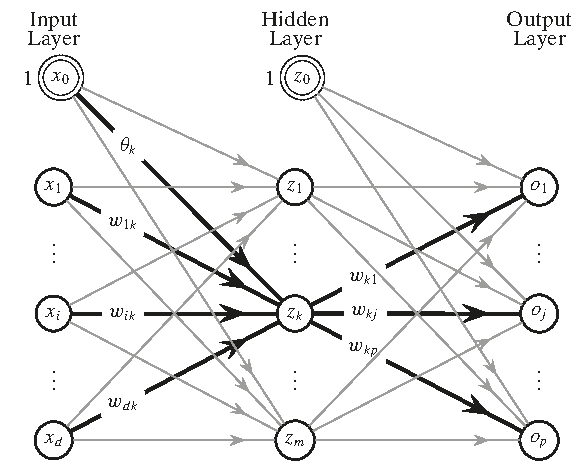
\includegraphics{pdf/NeuralNetwork.pdf}
  \caption{Exemplo de uma rede neural com uma camada escondida}
  \label{fig:neuralnetwork}
\end{figure}

O \textit{backpropagation} é um método usado em redes neurais artificiais para calcular um gradiente que é necessário no cálculo dos pesos a serem usados na rede. \textit{backpropagation} é uma abreviação para "a propagação retrógrada de erros", já que um erro é calculado na saída e distribuído para trás em todas as camadas da rede. \cite{backpropagation}\cite{rumelhart1986learning}

\begin{figure}[H]
  \centering
  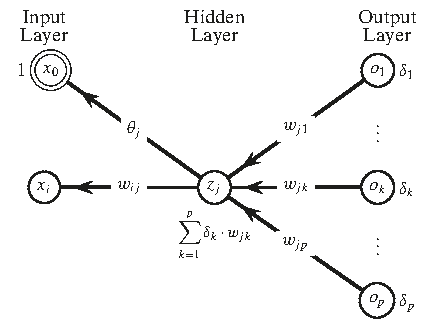
\includegraphics{pdf/backpropagation.pdf}
  \caption{Backpropagation dos gradientes da camada de saída para camadas antecessores}
  \label{fig:backpropagation}
\end{figure}

\subsection{Funções de ativação}

As funções de ativação utilizadas nas camadas escondidas é a \textbf{ReLU}, pois foi o que obtive os melhores resultados entre outras funções de ativação (\textit{sigmoid}, \textit{tanh}). Dois benefícios principais adicionais das ReLUs são a dispersão e uma \textit{reduced likelihood} do problema do \textit{vanishing gradient}\cite{maas2013rectifier}.

\[{\rm{ReLU(x) = }}\left\{ {\begin{array}{*{20}{c}}
x&{if\;x \ge {\rm{0}}}\\
0&{x < 0}
\end{array}} \right.\]

A camada de saída é composto por 3 neurônios contendo a função de ativação \textbf{Softmax}. Cada neurônio tem como saída a probabilidade do vetor de entrada pertencer a classe que este neurônio representa. \textit{Softmax} é uma generalização da \textit{sigmoid} ou função de ativação logística. Em resumo é uma saída exponencial normalizado com a soma de todas as saídas. Seja $c_j$ a j-ésima classe sendo que temos $K$ classes, temos:

\[P({c_j} = 1|\vect{x}) = {o_j} = \frac{{\exp [net_j]}}{{\sum\nolimits_{i = 1}^k {\exp [net_i]} }},\forall j = 1,2, \ldots ,K\]

\subsection{Função de Erro}

A função de erro escolhida $\vect{\delta}$ é a \textbf{Cross-Entropy Error} que é tipicamente utilizada com a função de ativação. \textit{Softmax}.

\[\delta _j^{h + 1} = {o_j} - {y_j}\]

Em que $y_i = 1$ se para i-ésima classe já rotulada e $y_i = 0$ para o restante. Com este vetor de erro é calculado a derivada da matriz $\textbf{f}$ das funções de ativação dos neurônios das camadas internas. Daí se tem a necessidade da função de ativação ser derivável.

\subsection{Treinamento}

Segue-se um pseudo-código generalizado com $h$ camadas escondidas.

\begin{figure}[H]
  \centering
  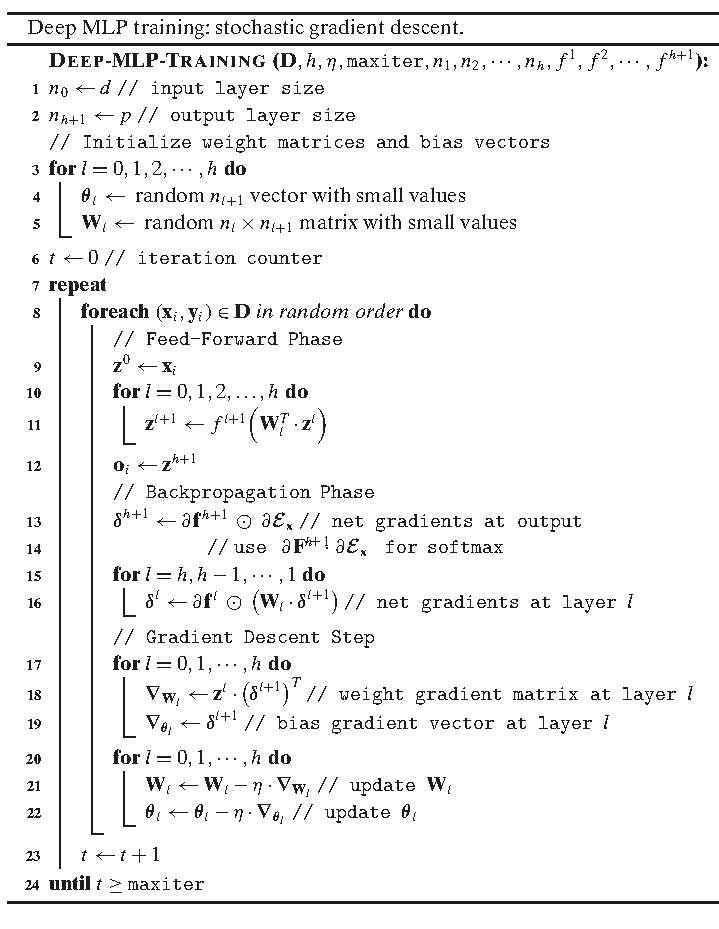
\includegraphics{pdf/mlp-alg.pdf}
  \caption{Multilayer Perceptron etapa de treinamento}
  \label{fig:mlpalg}
\end{figure}

\newpage
\section{Guia de experimentações}

Todas os experimentos utilizam os seguintes parâmetros:

\begin{itemize}
    \item $\rm{Learning Rate} = 0.01$
    \item Hidden Layers = Duas camadas escondidas de $16$ neurônios cada com função de ativação \textbf{relu}
    \item $\rm{Decaying Rate} = 0.0$
    \item $\rm{Epochs} = 100$
\end{itemize}

Com exceção quando é citado o próprio parâmetro mantendo os restantes constantes.

Na especificação é dado um guia de experimentações e vamos analisar cada questão. Todos os gráficos é o resultado
da média de 10 execuções para uma melhor confiabilidade de dados obtidos.

\begin{enumerate}
    \item O que acontece quando se aumenta o número de neurônios da camada escondida da rede? Isso afeta o
    número de épocas necessárias para convergência?
    
    \begin{figure}[H]
        \centering
        \includegraphics[width=1.0\textwidth]{pdf/"Guia001".pdf}
        \caption{Comparação de número de neurônios na camada escondida}
        \label{fig:compneurohidden}
    \end{figure}
    
    Vemos na Figura \ref{fig:compneurohidden} que a quantidade de neurônios impactam, mas após uma certa quantidade o ganho não é muito significativo. Verifica-se também que com uma quantidade maior de neurônios há uma convergência mais rápida exigindo uma quantidade menor de \textbf{epochs} para convergir.
    
    \newpage
    \item O que acontece quando se aumenta o número de camadas escondidas? O ganho no erro é grande o suficiente para justificar a adição de uma nova camada?
    
    \begin{figure}[H]
        \centering
        \includegraphics[width=1.0\textwidth]{pdf/"Guia002".pdf}
        \caption{Comparação de número de camadas escondidas}
        \label{fig:complayerhidden}
    \end{figure}
    
    A quantidade de camadas ajuda a combinar os limiares de características, o que pode ser melhor visualizado em um exemplo em 2D interativo na ferramenta Playground Tensorflow\cite{ANeuralN47:online}. No gráfico da Figura \ref{fig:complayerhidden} percebemos que uma maior quantidade de camadas da uma maior complexidade pois aumenta o espaço de busca dos pesos dos neurônios. Pode-se ver que o crescimento de acurácia não é tão suavizado quanto a quantidade menor de camadas.
    
    \newpage
    \item Qual o impacto da variação da taxa de aprendizagem na convergência da rede? Oque acontece se esse parâmetro for ajustado automaticamente ao longo das diferentes épocas?
    
    \begin{figure}[H]
        \centering
        \includegraphics[width=1.0\textwidth]{pdf/"Guia003a".pdf}
        \caption{Comparação de diferentes valores do Learning Rate}
        \label{fig:variationlr}
    \end{figure}
    
    Na figura \ref{fig:variationlr} destaca vários valores da taxa de aprendizagem através de $1000$ \textit{epochs}.
    
    Um valor muito baixo resulta em uma convergência muito lenta o que exige muitas \textit{epochs} para atingir um resultado satisfatório.
    
    Conforme os valores são incrementados, a convergência é melhorada mas em excesso é gerado um ruído que torna ruim o resultado da convergência. Com valor muito alto, a função de erro "passeia" dando saltos muitos altos o que pode nunca atingir o resultado ótimo ou piorar os pesos devido a imprecisão.
    
    \begin{figure}[H]
        \centering
        \includegraphics[width=1.0\textwidth]{pdf/"Guia003b".pdf}
        \caption{Comparação de decaimento da taxa de aprendizagem}
        \label{fig:decaylr}
    \end{figure}
    
    Na Figura \ref{fig:decaylr}, a taxa de aprendizagem inicial é $1.0$, um valor alto que se pode ver o efeito colateral quando $decay = 0.0$. E vemos que a o decaimento da taxa de aprendizagem ocasiona numa convergência forçada após algumas \textit{epochs}.
    
    \newpage
    \item Compare o treinamento da rede com \textit{gradient descent estocástico} com o \textit{mini-batch}.
    A diferença em erro de treinamento versus tempo computacional indica que qual deles deve ser utilizado?
    
    \begin{figure}[H]
        \centering
        \includegraphics[width=1.0\textwidth]{pdf/"Guia004".pdf}
        \caption{Comparação de SGD com mini-batch}
        \label{fig:compsgdminibat}
    \end{figure}
    
    A Figura \ref{fig:compsgdminibat} mostra o comportamento da acurácia quando com o SGD e mini-batch. Observa-se que com o SDG padrão há um decaimento da acurácia porque a atualização dos pesos é feita a cada avaliação de um elemento, enquanto o mini-batch o crescimento é suavizado pois a atualização é feita após $200$ avaliações se tornando o passo do gradiente mais generalizado.
    
    \newpage
    \item Qual a diferença do erro encontrado pela rede no conjunto de treinamento ou validação em relação ao erro encontrado no teste? Existe \textit{overfitting}? Como ele pode ser evitado?
    
    Como os dados são embaralhados na leitura do \textit{dataset}, é possível que a maior os dados da classe \textit{QSO} não estejam na partição de treinamento, ocasionando um erro na avaliação da classe de que não foi treinada.
    
    Se o \textit{overfitting} for causado pela rede, uma possível alternativa é a \textbf{Dropout Regularizattion}\cite{srivastava2014dropout}, em que durante o processo de treinamento, uma certa quantidade de neurônios são selecionados para serem desativados. Assim a rede fica mais robusta e evita o \textit{overfitting} ao mesmo tempo.
    
    A função está disponível na biblioteca padrão do Keras\footnote{\url{https://keras.io/layers/core/#dropout}}.
    
    \begin{figure}[H]
        \centering
        \includegraphics[width=1.0\textwidth]{pdf/"Guia006".pdf}
        \caption{Comparação utilizando Dropout Regularization}
        \label{fig:compdropout}
    \end{figure}
    
    Analisando este recurso na Figura \ref{fig:compdropout}, vemos que a acurácia da validação e do teste teve um bom ganho em que muitos casos tem a curva acima do valor de treinamento.
    
    \newpage
    \item A base com que você trabalhou é um pouco desbalanceada. Você pode tentar contornar esse problema usando a técnica de oversampling, ou seja, fazendo cópias dos exemplos das classes minoritárias para balancear melhor a base. Por exemplo, a classe QSO tem 412 exemplos, e a classe GALAXY 2501. De forma simples, você poderia fazer 6 cópias de cada exemplo da classe QSO, aumentando o número de exemplos dessa classe para 2472, e utilizando todos eles no treinamento da rede. Fazendo um oversampling das classes minoritárias e retreinando a rede com os melhore parâmetros encontrados, o erro diminuiu? Por quê?
    
    \begin{figure}[H]
        \centering
        \includegraphics[width=1.0\textwidth]{pdf/"Guia006".pdf}
        \caption{Comparação com a quantidade de QSO normalizado nos dados}
        \label{fig:compquantQSO}
    \end{figure}
    
    Pela Figura \ref{fig:compquantQSO} verificamos que a cruva de acurácia é normalizada após a aplicação do \textit{oversampling}.
    O \textit{oversampling} utilizado foi o sugerido na especificação de replicar 5 vezes a quantidade dos dados da classe \textbf{QSO}.
    
    O erro diminui pois na etapa de treinamento, as classes \textbf{QSO} ganham um maior peso devido pela quantidade maior que foi avaliada.
    
    \newpage
\end{enumerate}



\section{Conclusão}

O trabalho prático ajudou em aprender conteúdos profundos e novos que ainda era desconhecido para mim, como o \textit{Dropout Regularization}, que vem de paper recente de 2014 e foi incluído na biblioteca Keras após comprovada a sua eficácia. Também foi importante em verificar alguns das variações de parâmetros, o seu papel e seu comportamento na modelagem.

Por fim, o trabalho tem a sua importância em aprender os conceitos principais e por em prática em uma das principais bibliotecas do mercado.

% Can use something like this to put references on a page
% by themselves when using endfloat and the captionsoff option.

% ====== REFERENCE SECTION

% \begin{thebibliography}{1}

% IEEEabrv,
\bibliographystyle{IEEEtran}
\bibliography{IEEEabrv,Bibliography}
% \end{thebibliography}
% biography section
% 
% If you have an EPS/PDF photo (graphicx package needed) extra braces are
% needed around the contents of the optional argument to biography to prevent
% the LaTeX parser from getting confused when it sees the complicated
% \includegraphics command within an optional argument. (You could create
% your own custom macro containing the \includegraphics command to make things
% simpler here.)
%\begin{biography}[{\includegraphics[width=1in,height=1.25in,clip,keepaspectratio]{mshell}}]{Michael Shell}
% or if you just want to reserve a space for a photo:\

\vfill

% that's all folks
\end{document}


